\chapter{Irodalom}
\pagestyle{headings}

Ezen fejezetben diplomamunkám elméleti háttereként szolgáló szakirodalmi hivatkozásokat foglalnám össze. Nagyjából három jól elkülöníthető téma szakirodalmának vonatkozó részét tekintem át. Először a pásztázó mérőcsúcs mikroszkópia történetéről és működéséről írnék. A második alfejezetben a mikroelektródokra, különös tekintettel a referenciaelektródokra, a harmadikban pedig a galvanikus korrózióra térnék ki.

\section{Pásztázó mérőcsúcs mikroszkópia}

\subsection{Története}

%A mikroszkópos technikák kezdetleges kialakulása a 16. században kezdte meg forradalmát, mikor elkészítették az első mikroszkópot. Fejlődésük és kialakulásuk szorosan összefügg az orvostudomány előrehaladásával, hiszen a sejtek tanulmányozását szabad szemmel nem tudták megtenni. Az idő múlásával párhuzamosan jelentek meg az eltérő típusú mikroszkóp családok: a fénymikroszkóp, elektronmikroszkóp és ennek egy alfaja, a pásztázó elektronmikroszkóp. Ez utóbbi csoportra térnék ki részletesebben dolgozatomban \cite{masters2008history}. 



A következő néhány bekezdésben röviden kitérek pár mérföldkőnek számító technikára, különös tekintettel a dolgozatom szempontjából fontosabbakra. A pásztázó mérőcsúcs mikroszkópia (Scanning Probe Microscopy, SPM) története az irodalom szerint a pásztázó alagút mikroszkóp (Scanning Tunneling Micsocopy, STM) kifejlesztésével kezdődött 1981-ben, az IBM svájci laboratóriumában dolgozó Gerd Binning és Heinrich Rohrer munkájának köszönhetően \cite{binnig1982tunneling}. A technika lényege az alagúthatás, melyet a minta és a rendkívül hegyes mérőcsúcs között létesített nagy feszültség létrehozásával érnek el. A minta és a mérőcsúcs közötti távolság éppen úgy van megválasztva, hogy az elektronok számára pusztán energiájuk alapján egy áttörhetetlen potenciálgátat jelentsen. Az alagúthatás jelenségének köszönhetően azonban ezt a potenciálgátat át tudják törni egy bizonyos távolságon belül. A távolságot a mérés során úgy változtatja egy automatikus visszacsatolási kör, hogy ez éppen bekövetkezhessen. A mérőcsúcs tehát pontosan követi a minta topográfiáját. Mivel ez a mérés során folyamatosan ismert, ebből és az X-Y koordinátákból a minta magasságtérképe kirajzolható rendkívül nagy pontossággal. A technikával akár egyedi atomokat is láthatunk. A technika olyan nagy jelentőségűnek bizonyult, hogy már 1986-ban Nobel díjat adományoztak a két kutatónak.

Az atomerő mikroszkópot (Atomic Force Microscopy, AFM) ugyanebben az időben, szintén Binning és társai találták fel, majd néhány évre rá sikeresen kivitelezték a technikát a gyakorlatban is \cite{binnig1986atomic}. Az STM-hez hasonlóan ez a mérőtechnika is piezomotorokat használ a nagy felbontású képalkotáshoz, de ez a módszer határozottan szofisztikáltabb működésű az előzőnél. Szigetelő és vezető tulajdonságú felületek esetén is közel atomi szintű felbontást nyújt. Egy lézernyaláb visszaverődési szögének mérésén alapul. A mérőcsúcs egy mikroméretű tartókaron helyezkedik el, ami néhány atomnyi távolságra helyezkedik el a mintától, ezért elhajlik a mintán és a mérőcsúcson lévő atomok kölcsönhatása végett. A lézernyalábot a mérőcsúcsra mintával ellentétes oldalán lévő mikroméretű tükörre vetítjük, majd ez egy diódasorra veri vissza a ráirányított sugarat. A mérőcsúcs bizonyos mértékben el fog hajlani, a mintán fellelhető topográfiai elváltozások következtében, emiatt pedig megváltozik a lézernyaláb visszaverődési szöge. Az egyes pozícióknál mért magasságra a lézernyaláb beesési szögéből tudunk következtetni. A tartókar mozgatása nagyon kicsi erőt igényel, innen ered a technika neve. Érzékenysége sok újfajta alkalmazásnak nyitott teret, mint például szigetelő és vezető anyagok atomi szintű vizsgálata \cite{salapaka2008scanning}.

Megjegyezném azonban, hogy a dolgozatomban is alkalmazott pásztázó referencia elektród technikát (Scanning Reference Electrode Technique, SRET) már 1979-ben kifejlesztette és sikerrel alkalmazta Hugh Isaacs \cite{isaacs1981scanning}. Az említett kutató főleg korrózióval foglalkozott, és a SRET-et egy korróziós probléma megoldására fejlesztette ki. A mérés során egy mikroméretű referenciaelektródot mozgatunk, amivel a lokális korrózió során a fém felületének közelében valós időben mérhetjük a potenciált, a folyamat megzavarása nélkül. Ez tehát egy nem invazív elektrokémiai módszer. Fémek korróziója során potenciál mezők keletkeznek az elektrolitban, mivel a katódos oldal felszíne felé elektromos áram folyik az anódos területről. A technika azonosítja ezen területeket valós időben. Rendkívül kis potenciálváltozásokat is képes detektálni az aktív minta felületén. Hasznos eszköznek bizonyult az \emph{in situ} korróziós vizsgálatoknál, mint például fémbevonatok delaminációja és különböző ötvözetek, fémek korróziós viselkedésének vizsgálata \cite{maile2000evaluation, cui2001use}.

Egy másik rokon technikát, a pásztázó vibráló elektród technikát (Scanning Vibrating Electrode Technique, SVET) már 1974-ben használták az extracellurális ionmozgásokkal asszociálható áramerősségek mérésére \cite{jaffe1974ultrasensitive}. Az 1980-as években kezdte Hugh Isaacs különböző korróziós folyamatok vizsgálatához továbbfejleszteni és alkalmazni \cite{isaacs1988initiation}. Működése során az oldatban méri a minta felett a helyi áramerősség sűrűségének eloszlását, és ezzel feltérképezi a felületen lezajló elektrokémiai folyamatokat \emph{in situ}, miközben kialakulnak. Mivel a mért áramerősség függ a reakció sebességétől, a technika kvantitatív. Mérőcsúcsként a mintára merőlegesen rezgő mikroméretű platina pálcát használ, amivel az elektromos potenciált mérjük a rezgőmozgás két szélsőhelyzetében egy ún. ,,lock-in'' erősítő segítségével. A technika szorosan összefügg a SRET-el, tulajdonképpen ez annak egy továbbfejlesztett változata. 

A korábban említett SRET technika előnyének mondható a SVET-el szemben, hogy non-invazív technika, tehát a korróziós vizsgálatokban a folyamatok megzavarása nélkül térképezhetjük fel a céltárgy anódos és katódos részeit. Az elektrolit oldatot se keveri olyan mértékben a vizsgálat során. A SVET azonban egy érzékenyebb technika, ami a vibráló mérőcsúcsnak és az emiatt javuló jel-zaj viszony arányának köszönhető. SRET-el az elektrokémiai folyamatban kialakuló potenciál különbségeket mérjük a minta felett az elektrolit oldatban, míg a SVET az áramerősség sűrűséget vizsgálva ad információt és alkot képet az oldatban lezajló elektrokémiai folyamatokról. A két információ azonban ekvivalensnek mondható, hiszen az Ohm--törvényen keresztül kapcsolatban állnak egymással.

Elektroanalitikai szempontból az 1980-as években mérföldkövet jelentett, mikor Allen J. Bard és csoportja lefektették az elméleti és gyakorlati alapjait a pásztázó elektrokémiai mikroszkópiának (Scanning Electrochemical Microscopy, SECM) \cite{bard1989scanning,bard1990scanning}. Megjegyzendő azonban, hogy három évvel korábban Engstrom már végzett hasonló méréseket \cite{engstrom1989scanning}. Egy mikroelektróddal pásztázott egy másik elektródot, melyeket egy bipotenciosztáttal polarizált. Így ,,generáló--gyűjtő'' módban alkalmazhatta az elektródokat és a mikroméretű mérőcsúcshoz diffundált a másik elektród által generált anyag. Mikromanipulátort használt a mozgatásához. Általánosságban véve a módszer lényege, hogy egy mikroelektródot alkalmazunk mérőcsúcsként, melynél a hegyen is elektrokémiai reakció játszódik le, és ezzel pásztázzuk a vizsgálandó mintát. A mikroelektród a mérés során polarizálva van egy potenciosztát segítségével, tehát a mérőcsúcs tulajdonképpen egy amperometriás mérőkör munkaelektródja. 

Korábban említett közleményekből idézve megemlítenék még egy ismert jelenséget, ami jelentős a felületek vizsgálata során, ez pedig a visszacsatolás (feedback) jelensége (\ref{fig:feedback}. ábra). Megkülönböztetünk pozitív és negatív visszacsatolást. Ha a mérőcsúcsot közelítjük a céltárgyhoz, és ez a távolság eléri merőlegesen a minta felületétől számítva a 3d-nél kisebb értéket (d alatt az elektród aktív felületének átmérőjét értjük), a mért áramerősség a minta felszínének jellegétől függően változni fog. 

Vezető felület esetén pozitív visszacsatolás tapasztalható. Minél közelebb jutunk a felülethez, annál nagyobb áramerősséget detektál a műszer a tömbfázisban mérthez képest.  Magyarázata, hogy a vezető felület és a mérőcsúcs között kialakult pozitív visszacsatolási kör egyre rövidebbé válik, ahogy közeledünk a minta felületéhez. Vagyis reverzibilis reakció esetén, visszaoxidálódik eredeti formájába a mérőelektród által redukált anyag. 

Negatív visszacsatolás esetén az áramerősségben folyamatos csökkenést detektálunk, ahogy a mérőcsúcs közelebb ér a felszínhez. Ezt szigetelő tulajdonságú felszínek vizsgálata során figyelhetjük meg, aminek oka, hogy a mérőelektród aktív felületénél nullára csökken az oxidálható anyag koncentrációja. A csökkenő távolság megakadályozza, hogy átalakítható anyag diffúzió révén pótolható legyen. Emiatt a detektált áramerősség is nullára csökken, vele arányosan.

Az említett 3d távolság felett ezeket az összefüggéseket az áramerősségben és a mért távolságban nem tapasztaljuk. A jelenséget lehet használni a minta--mérőcsúcs távolság beálltására, hiszen ha ismerjük a 3d távolságot és ismerjük az elektród átmérőjét (d), akkor kiszámolható az éppen aktuális minta--elektród távolság is.

\begin{figure}
\centering
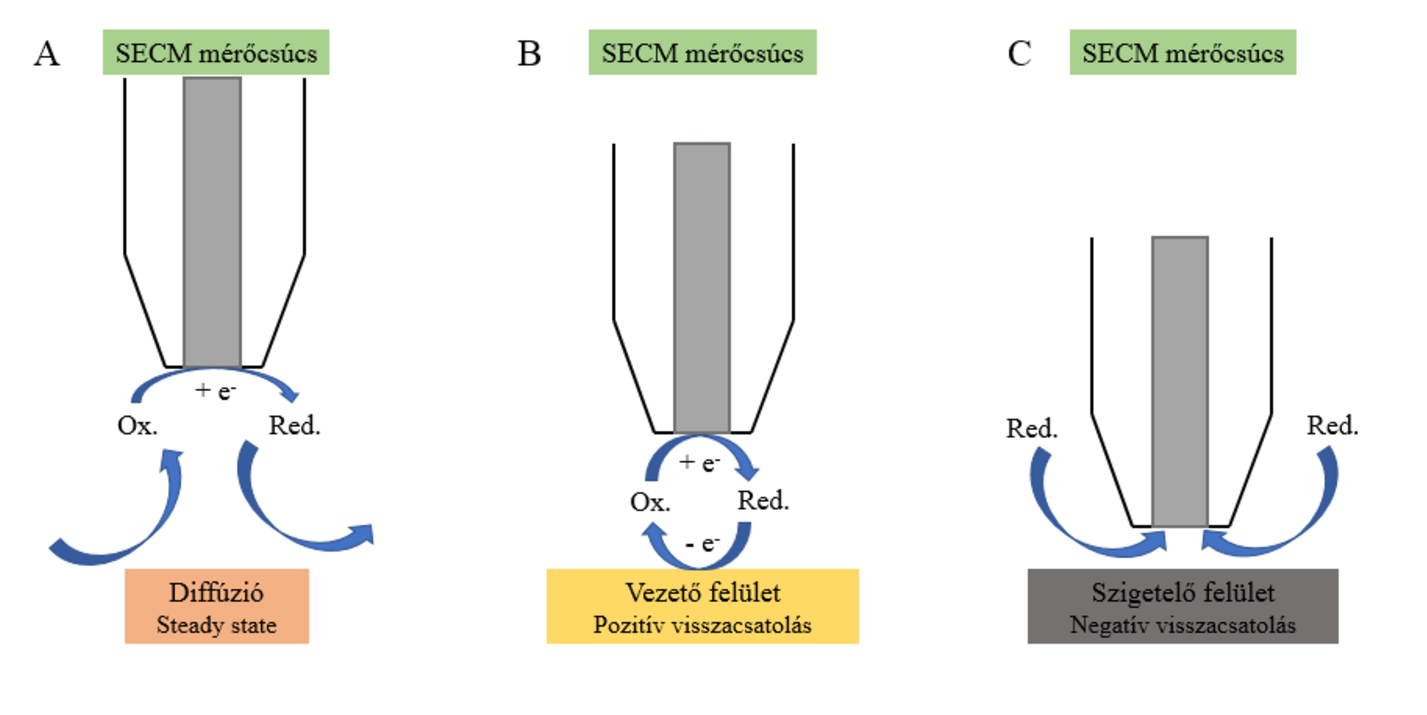
\includegraphics[width=0.8\textwidth]{img/feedback.eps}
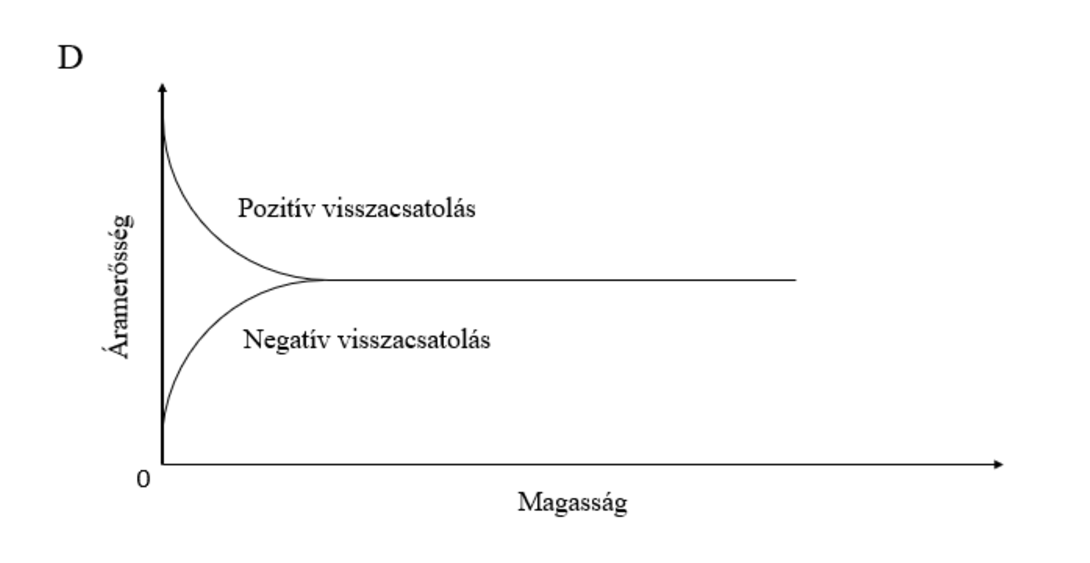
\includegraphics[width=0.8\textwidth]{img/feedback2.eps}
\caption{Visszacsatolás jelensége:
A: 3d magasság felett tömbfázisú áramerősség
B: vezető felület felett pozitív
C: szigetelő felett negatív visszacsatolás
D: áramerősség a magasság függvényében. A magasság a mérőcsúcs vége és a céltárgy felszíne közti távolságra értendő}
\label{fig:feedback}
\end{figure}

Eredetileg amperometriás detektálásokra lett kifejlesztve a PEKM technika. Nagy hátránya, hogy kevés kémiai információt ad. Nem sokkal később viszont megjelent a potenciometriás változat, Nagy Géza és Benjamin Horrocks kutatásainak köszönhetően, melyben a hidrogénion aktivitást térképezték \cite{horrocks1993scanning}. Potenciometriás ionszelektív elektród mérőcsúccsal lehetővé vált tehát a tényleges kémiai környezet feltérképezésére is. Manapság egyre elterjedtebben használják a technikát, mivel kiválóan alkalmazható különböző ionok szelektív térképezésére megfelelő ionszelektív mérőcsúcs alkalmazásával \cite{souto2011spatially}. Ez pedig a korróziós vizsgálatok során rendkívül előnyös tulajdonság \cite{souto2013spatially}. A technika kifejlesztésekor már rendelkezésre állt makroméretű ionszelektív elektródok egész sora, többek között egy magyar kutatócsoportnak köszönhetően, Pungor Ernő vezetésével \cite{pungor1978ion,pungor1998theory}.

\subsection{Működése}
A pásztázó mérőcsúcs mikroszkópos módszerek alapvetően eltérnek a hagyományos mikroszkópos módszerektől. Fénymikroszkóp esetében például a teljes látómezőről egyidejűleg kapunk adatokat, az összes mérési ponthoz tartozik egy érzékelő, mint például a CCD mátrixban az egyes pixeleknek megfelelő fényérzékeny elemek. Ezzel szemben a pásztázó mikroszkópos technikák közös tulajdonsága, hogy a képalkotás során minden egyes ponton ugyanazzal az érzékelővel mérjük a vizsgált paramétert. A szenzort sorban egymás után pozícionáljuk a vizsgálni kívánt minta feletti pontrendszer minden egyes pontjához. A pontrendszer minden egyes pontján megállítjuk a szenzort és egy lokális mérést végzünk. A mérés eredményét eltároljuk a mérés koordinátáival együtt. A kapott adathalmazból egy képet tudunk készíteni, ábrázolva a mérések eredményét a koordináták függvényében. A technika nagyon sokoldalú, hiszen kicserélve a mérőcsúcsot vagy a detektálás elvét, rendkívül változatos méréseket végezhetünk el. 

A SPM alapja tehát a raszteres képalkotás. Működését a SECM példáján mutatnám be. A mérőcsúcsot, ami jelen esetben egy mikroelektród, mozgatjuk egy előre meghatározott algoritmus szerint, a vizsgálandó minta felett (\ref{fig:PEKM}. ábra). A mikroelektród egy mikromanipulátorhoz van rögzítve, amit egy számítógépes programmal egyszerűen kezelhetünk. Általában meanderező mozgást követ a szoftver, de lehet például vonalpásztázást és összetett vonalpásztázást is alkalmazni algoritmusként \cite{kiss2014new}. A mérések előtt kell megadnunk a paramétereket a programnak (mozgás, lépésköz és ennek ideje, intervallum). Megkülönböztetünk amperometriás és potenciometriás méréseket. Amperometriás mód esetén a cella egy mérőelektródból, egy referencia elektródból és egy segédelektródból áll. A mérőelektródot mozgatjuk, míg a referencia- és segédelektród a pásztázási területtől odébb helyezkedik el, hogy ne zavarja a mérést. Potenciometriás módban pedig egy referencia elektródból és egy ionszelektív elektródból épül fel a cella, és az ionszelektív elektród potenciálját mérjük a referencia elektródhoz képest.

\begin{figure}
\centering
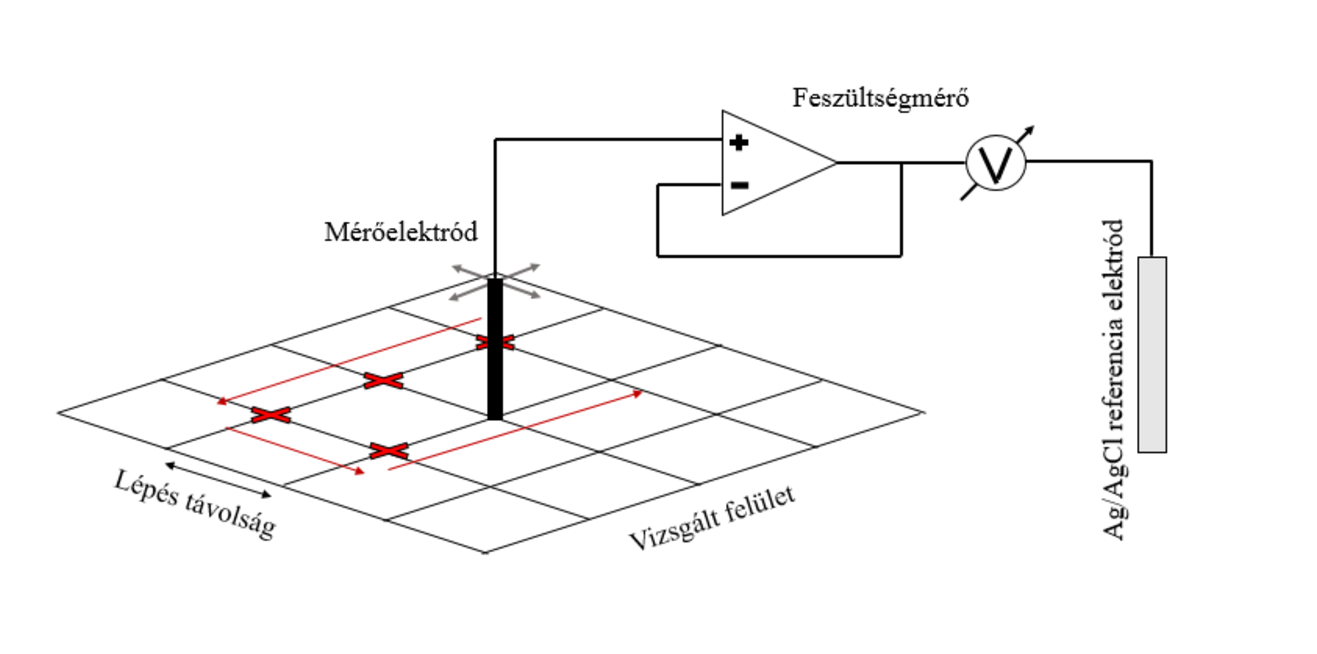
\includegraphics[width=0.8\textwidth]{img/spm.eps}
\caption{Pásztázó elektrokémiai mikroszkóp működésének szemléltetése.}
\label{fig:PEKM}
\end{figure}

\section{Referenciaelektródok}

Az elektroanalitikában elengedhetetlen mérőeszközök az elektródok. A potenciometriás elektródokat általában az alábbi módon osztályozzuk \cite{kalman2002az}:

\begin{enumerate}  
    \item Ionszelektív elektródok
      \begin{enumerate}
	\item Üvegelektród
	\item Nem üvegalapú membrán-elektród
	\item Folyadékmembrán-elektród
	\item Enzimelektród
	\item Gázelektród
	\end{enumerate}
    \item Redoxi elektródok (Zérus fajú)
    \item Elsőfajú és másodfajú elektródok
\end{enumerate}

Ionszelektív elektródok együttes elvi alapja az ioncsere-egyensúly. Az oldatbeli koncentrációkat vizsgáljuk egy ismert koncentrációjú standardhoz viszonyítva. A két koncentráció különbség, illetve a mért potenciálkülönbség alapján számíthatjuk ki az elsődleges ion aktivitását. Ezek az elektródok az esetek többségében egy adott ionra szelektívek, az oldatban előforduló zavaró ionok hatása ellenében is szelektív választ adnak. A detektált potenciál érték és a jelenlévő összes ion aktivitásának kapcsolatát a Nikolszkij--Eisenmann-egyenlet írja le:

\begin{equation}
E = E^\theta + \frac{0,059}{n_i}\lg \Big (a_i + K_{ij} a_j^\frac{n_i}{n_j} \Big )
\label{eq:nikolszkij}
\end{equation}

ahol a$_i$  a mérendő és a$_j$ a zavaró ionok aktivitása, n$_i$ és n$_j$ ezen ionok töltése, K$_{ij}$ az ionszelektív elektród szelektivitási tényezője, E az ionszelektív elektródpotenciál, E$_0$ pedig a standard elektródpotenciál.

A redoxi elektródok elvi alapja az elektroncsere egyensúly. Inert nemesfém, platina általában, vagy grafitelektródok biztosítják az elektronátmenetet. A potenciált a Nernst--egyenlet segítségével írhatjuk le:

\begin{equation}
E = E^\theta + \frac{0,059}{n}\ln \frac{[ox]}{[red]}
\label{eq:nernst}
\end{equation}

Elsőfajú elektródok egy elemből vagy fémből és saját ionját oldott állapotban tartalmazó oldatokból állnak, és a felületükön fellépő potenciálváltozás leírható a Nernst--egyenlettel. Általában munkaelektródként használatosak az ilyen típusú elektródok.

Másodfajú elektródok, hasonlóan az elsőfajúhoz, egy reverzibilis fémelektródot tartalmaznak, és ez valamely rosszul oldódó sójával és a só anionjának telített oldatával van egyensúlyban. A fém feladata, hogy az elektronburkába befogadja vagy innen elektront szolgáltasson az elektród működése közben elnyelt vagy keletkező elektronokat. Mivel egy rosszul oldódó csapadékos rendszerbe merül a fém, aminek oldata telített, így az ionkoncentráció szorzata is állandó érték. A só anionját tartalmazó telített oldat pedig a megfelelő ionkoncentrációt és a jó elektromos vezetést biztosítja. Ezek az elektródok főként referencia elektródnak használhatóak kitűnően, kis polarizálhatóságuknak köszönhetően.

Referencia elektródoknak nevezzük azon elektródokat, melyek stabil és ismert elektród potenciállal rendelkeznek \cite{allen2001electrochemical}. A magas stabilitást úgy érhetjük el, ha egy redox rendszert alkalmazunk állandó (pufferelt vagy telített) koncentrációjú reagensekkel a redoxi reakcióban. Leggyakoribb alkalmazási módja, mikor félcellaként használjuk egy elektrokémiai cellában. Így a cella másik felének a potenciálját meg tudjuk határozni. Gyakorlatban főként az Ag/AgCl és Hg/Hg$_2$Cl$_2$ elektródok használatosak. 

\subsection{Felépítésük}

Az Ag/AgCl referencia elektróddal szemléltetném a felépítést \cite{janz1968silver}. Az elektródban egy ezüstszál található, amit ezüst-klorid von be, és telített klorid-ion oldatba merül. Ilyen lehet például ismert koncentrációjú KCl-oldat, és ez addig telített az AgCl-ra, míg az elektródon szilárd ezüst-klorid fellelhető.


Általános felépítése ábrázolva : Ag(sz) | AgCl(sz) | Cl$^-$(aq)


A benne lévő csapadék anionjára nézve reverzibilis elektródként működik. Vagyis az elektrolit oldatban állandó értékű ionkoncentráció következménye, hogy az elektród potenciálja is állandó értéket mutat. Így tehát, ha egy rendszer koncentrációváltozását kívánjuk nyomon követni, akkor a referencia elektródot egy mérőelektróddal kapcsoljuk össze, és a két elektród közötti potenciálkülönbség a mérőelektród potenciál változását fogja mutatni \cite{harrisquantitative}.

\section{Galvanikus korrózió}

Általánosságban elmondható, hogy a galvanikus korrózió olyan elektrokémiai folyamat, melyben az egyik fém korrodálódik, amikor ugyanazon elektrolit oldatban a másikkal elektromosan kapcsolva van. A különböző fémek vagy ötvözetek eltérő elektród potenciállal rendelkeznek, és amikor ugyanazon elektrolitba közvetlen kapcsolatba kerülnek, a reaktívabb fém anódként, a kevésbé reaktív katódként viselkedik. Az ok, ami miatt az anódos fém gyorsabban korrodálódik, mint általában, az elektród potenciál különbség a két elektród közt lejátszódó reakcióban. A reakcióban az anód az elektrolitba oldódik és a katódon a korrózió mondhatni gátolva van. Az elektrolit jelenléte kulcsfontosságú a galvanikus korrózió kialakulásához, mivel az ionos migrációt segítik elő. Az ionok pedig e során megakadályozzák a töltés felgyülemlést, ami a reakciót megállítaná \cite{fontana2018corrosion}. 

Előzőleg már említett közlemények alapján, elmondható, hogy vizes oldatban a fémek korróziója egy elektrokémiai folyamat, mely során az anódos fém oxidálódik, a katódos fémen redukció zajlik le \cite{isaacs1981scanning}. A fémes fázisban áramló elektronok nem mutatnak jelentős mértékű potenciálkülönbséget, a fém kis ellenállása miatt. Bármely elektrokémiai reakcióban a legnegatívabb félcella általában oxidálódik, és a legpozitívabb vagy legnenemesebb félcella pedig általában redukálódik. A szabály szerint a hidrogénnél negatívabb potenciálú fémek korrodálódnak savakban. A redox sor tetején lévő fémek, pl. platina, arany rendkívül inertek, így csak nagyon erőteljes oxidáló ágensekkel korrodálódnak. 

Sok előnyös tulajdonságaik ellenére, a fémek és ötvözeteik spontán korrózión mehetnek keresztül bizonyos körülmények közt, főleg igaz ez vizes környezetben \cite{izquierdo2013potentiometric}. Példának véve egy vas-magnézium galvánpáron ismertetném a folyamatot. A magnézium aktív természete lehetővé teszi, hogy feláldozható anódként védelmet nyújtson más fémeknek (\ref{fig:corrosion}. ábra). Az oldódás az anódként viselkedő magnézium oxidációjának eredményeként jön létre, ahol a folyamatot a katód környezetében végbemenő redukció tartja fenn. A vas korróziója megáll, míg a magnézium oldódik, ezzel lokális változásokat idéz elő a folyadék fázisban, az ion és molekuláris koncentrációkban. Mg$^{2+}$- ionokat produkál az anódos oldalon, miközben két elektront lead a katódos oldalon lévő vasnak. A katódos oldalon pedig oxigén vagy hidrogén-ion elnyelés történik, a magnézium által leadott két elektron igénybevételével. Ezek helyi pH változásokat idéznek elő, ami egyébként a korrodáló rendszerek egyik fontos ismertetőjegye. Ezért tanulmányozható a rendszer amperiometriásan és potenciometriásan, utóbbinál ionszelektív mikroelektródokkal.

\begin{figure}
\centering
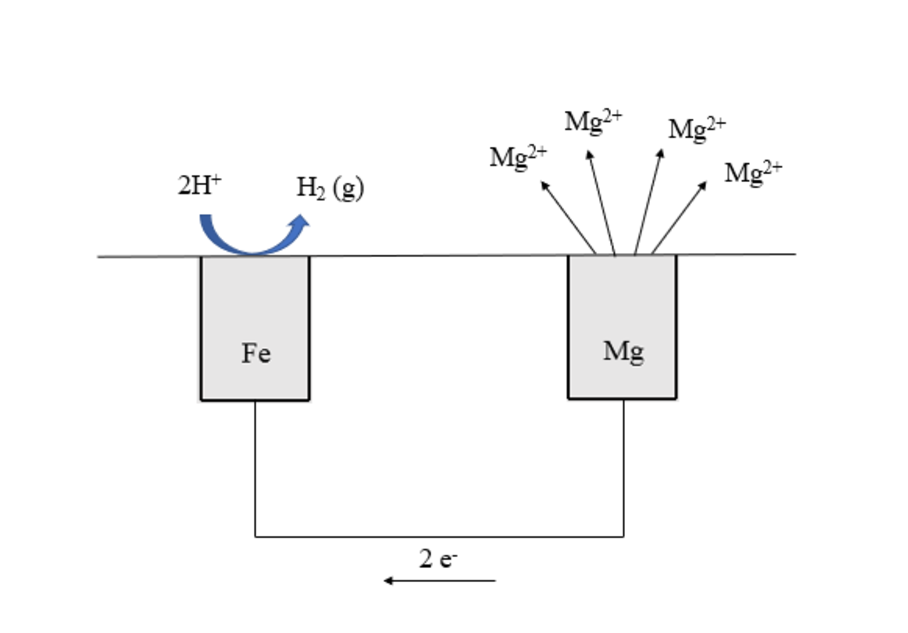
\includegraphics[width=0.6\textwidth]{img/corrosion.eps}
\caption{A galvanikus korrózió és az áldozati anód jelenségének szemléltetése a példa alapján.}
\label{fig:corrosion}
\end{figure}

Diplomamunkám szempontjából fontos megemlítenem a korróziós reakciók során kialakuló elektromos mezőt is \cite{morley1994principles}. Ez minden elektromos töltést körbevesz és a közegben a töltések egymásra hatást gyakorolnak, taszítják vagy vonzzák egymást. Faraday megfogalmazása szerint a töltéssel rendelkező részecskék maguk hozzák létre ezt a mezőt, mely segítségével erőt képesek kifejteni egymásra. Matematikában ezt egy vektor mezőként definiáljuk, mely a tér minden egyes pontjához egy töltést rendel, amire adott erő hat (vagyis iránnyal és nagysággal is rendelkezik) \cite{purcell2013electricity}. Coulomb törvénye szerint a stacionárius töltések esetében az elektromos mező az adott töltés távolságának négyzetével fordítottan arányosan és a töltéssel arányosan változik. Tehát, ha a töltést duplázzuk, az elektromos mező is ennyivel nő, ha pedig a távolságot vesszük kétszeresnek, a mező ereje azon az adott pontban negyede lenne. Mértékegysége a V/m, ami a N/C-al ekvivalens. Elektromos potenciál mérése esetében a referencia elektródhoz képest mérünk potenciálkülönbséget. Így a közeg két pontjában mért potenciál értéket nevezzük potenciálkülönbségnek, az adott pontok közt. Fizikában a következőképpen definiáljuk, a Nabla-operátor alkalmazásával:
\begin{equation}
{E} = - \nabla \Phi - \frac{ \partial \mathbf{A} }{ \partial t}
\label{eq:field}
\end{equation}
Ahol $\nabla \Phi$ az elektromos mező gradiense és $\frac{ \partial \mathbf{A} }{ \partial t }$ az A idő szerinti első parciális deriváltja. A Nabla egy matematikában használt vektor differenciál operátor. Alkalmazhatjuk egy dimenzióban, mely esetben egy adott funkció standard deriváltjára utal. Több dimenzióban, vagyis egy mezőre alkalmazva, jelölheti bármely három operátort (grádiense, divergenciája vagy rotációja egy vektor mezőnek). Ez utóbbira a következőképp írható fel:

\begin{equation}
{\nabla 3=\left(\begin{matrix}
\frac{\partial E}{\partial x} , 
\frac{\partial E}{\partial y} ,
\frac{\partial E}{\partial z}
\end{matrix}\right)}
\label{eq:nabla}
\end{equation}

Korábban már említett közleményben az Ohm-törvény és a Laplace-egyenlet segítségével írható fel a potenciál eloszlás és áramerősség \cite{isaacs1981scanning}:
\begin{equation}
{i} = - \kappa \nabla E
\label{eq:field1}
\end{equation}
ahol E a potenciál, i az áramsűrűség és $\kappa$ az oldat vezetőképessége. Ez függ az anódos és katódos környezet polarizációs tulajdonságaitól. Ha egyik oldalon magas polarizáltságot mérünk, alacsony értékű áramerősséget detektálhatunk az oldatban. Vagyis a katód és anód között kis potenciálváltozás történik. Magas áramerősség esetében pedig nagyobb potenciálváltozások mérhetőek.

Az előzőleg példaként felvázolt galvánpáron ismertetve, egy erős elektromos mező alakul ki köztük (\ref{fig:field}. ábra), mely a két eltérő fém potenciálkülönbsége eredményeképp jön létre \cite{kiss2017effect}. Ez a felület és a galvánpár közt oszlik el és közvetlen hatással van a mérőelektród potenciáljára is. Tehát a mért potenciál ennek kettőnek az összege. Némely esetben az elsődleges ion aktivitásának potenciálkülönbségét is meghaladhatja egy erősebb elektromos mező potenciálkülönbsége. Emiatt nem kívánt módon zavarhatja a detektált jelet és alá- vagy túlbecsülhetjük az elsődleges ion aktivitását. Viszont, ha az elektródok helye közti potenciálkülönbséget hozzáadjuk az elektród hegyénél mért elsődleges ion aktivitásához, a következő egyenletet kapjuk:

\begin{equation}
\Delta E = E_M - E_R (\Phi_M - \Phi_R) 
\label{eq:field1}
\end{equation}

ahol $\Delta$E a mért potenciál különbség, E$_R$ a referencia elektród potenciálja, $\Phi_R$ és $\Phi_M$ a helyi potenciáljai az elektromos mezőnek. 

\begin{figure}
\centering
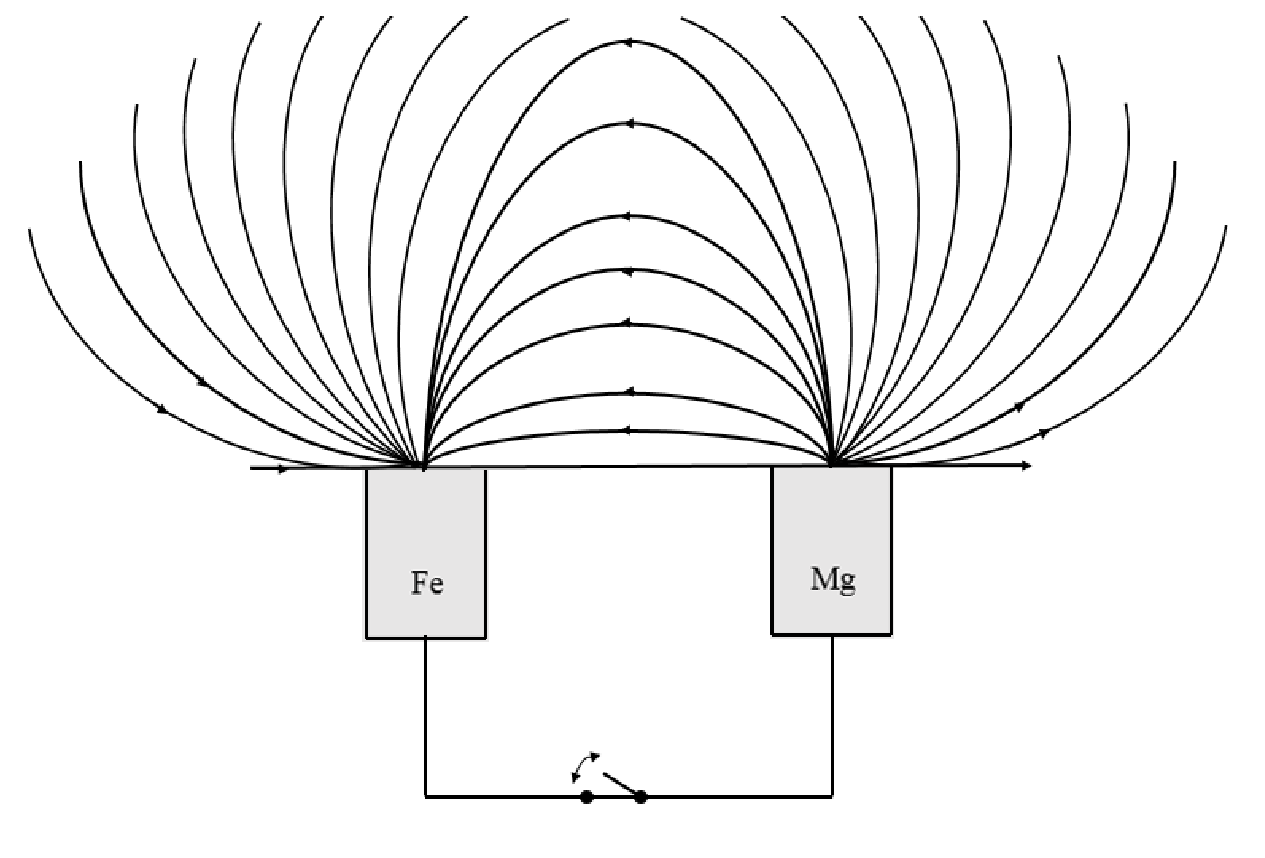
\includegraphics[width=0.6\textwidth]{img/field.eps}
\caption{Az eltérő fémek felszíne között kialakuló elektromos mező sematikus szemléltetése.}
\label{fig:field}
\end{figure}

Kísérleti bizonyítások alapján ez az effektus csökkenthető. Egyik megoldás a problémára, hogy ha a referencia- és mérőelektródot közel helyezzük egymáshoz. Így az elektromos mező, ami a két komponens által érzékelhető, egyenértékű, tehát kioltják egymást. Másik megoldásként elektromos relét alkalmazhatnánk kapcsolóként a galvánpár közt. Ezzel szétkapcsoljuk őket egy nagyon rövid időre, amíg a mérést végezzük.




